\documentclass[12pt,a4paper,oneside]{article}

\usepackage[utf8]{inputenc}
\usepackage[portuguese]{babel}
\usepackage[T1]{fontenc}
\usepackage{amsmath}
\usepackage{amsfonts}
\usepackage{amssymb}
\usepackage{graphicx}
\usepackage{xcolor}
\usepackage{multicol}
% Definindo novas cores
\definecolor{verde}{rgb}{0.25,0.5,0.35}

\author{\\Universidade Federal de Jataí (UFJ)\\Bacharelado em Ciência da Computação \\Linguagens Formais e Autômatos \\Esdras Lins Bispo Jr.}

\date{07 de dezembro de 2018}

\title{\sc \huge Prova (Parte 2)}

\begin{document}

\maketitle

{\bf ORIENTAÇÕES PARA A RESOLUÇÃO}

\small
 
\begin{itemize}
	\item A avaliação é individual, sem consulta;
	\item A pontuação máxima desta avaliação é 10,0 (dez) pontos, sendo uma das 06 (seis) componentes que formarão a média final da disciplina: quatro mini-testes (MT), uma prova final (PF), exercícios-bônus (EB) e exercícios aplicados em sala de aula pelo método de Instrução pelos Colegas (IpC);
	\item A média final ($MF$) será calculada assim como se segue
	\begin{eqnarray}
		MF & = & MIN(10, S) \nonumber \\
		S & = & [(\sum_{i=1}^{4} max(MT_i, SMT_i ) + PF].0,2  + EB + IpC\nonumber
	\end{eqnarray}
	em que 
	\begin{itemize}
		\item $S$ é o somatório da pontuação de todas as avaliações, e
		\item $SMT_i$ é a substitutiva do mini-teste $i$.
	\end{itemize}
	\item O conteúdo exigido desta avaliação compreende o seguinte ponto apresentado no Plano de Ensino da disciplina: (3) Autômatos Finitos Não-determinísticos, (4) Expressões Regulares, (5) Linguagens não-regulares, (6) Gramáticas Li\-vres-do-Contexto, (7) Autômatos com Pilha, e (8) Linguagens Não-Livres-do-Contexto.
\end{itemize}

\begin{center}
	\fbox{\large Nome: \hspace{10cm}}
\end{center}

\newpage

\begin{enumerate}
	
	\section*{Mini-Teste 3}
	
	\item (5,0 pt) {\bf [Sipser 1.20]} Para cada uma das seguintes linguagens, dê duas cadeias que são membros e duas cadeias que não são membros - um total de quatro cadeias para cada linguagem. Assuma que o alfabeto é $\Sigma = \{a,b\}$ em todos os casos.
	\begin{enumerate}
		\item (2,0 pt) $aba \cup bab$ 
		
		\vspace*{0.3cm}
		
		{\color{blue} {\bf Resposta:} Membros - $aba$ e $bab$ / Não-membros - $\epsilon$ e $a$.}
		
		\item (3,0 pt) $(a \cup ba \cup bb)\Sigma^*$
		
		\vspace*{0.3cm}
		
		{\color{blue} {\bf Resposta:} Membros - $a$ e $ba$ / Não-membros - $\epsilon$ e $b$.}
	\end{enumerate}
	
	\item (5,0 pt) {\bf [Sipser 1.29 (b)]} Use o lema do bombeamento para mostrar que $A = \{\omega \omega \omega$ | $\omega \in \{a, b\}^* \}$ não é regular.
	
	\vspace*{0.3cm}
	
	{\color{blue} {\bf Resposta:} Vamos supor, por um momento, que $A$ seja regular. Seja $p$ o comprimento do bombeamento dado pelo lema do bombeamento. Escolha $s$ como a cadeia $a^pba^pba^pb$. Como $s$ é um membro de $A$ e $s$ tem comprimento maior do que $p$, o lema do bombeamento garante que $s$ pode ser dividida em três partes, $s = xyz$, satisfazendo as três condições do lema. Mostramos que isso é impossível.
		
		A condição 3 é crucial, pois sem ela poderíamos bombear $s$ se fizéssemos $x$ e $z$ iguais a cadeia vazia. Com a condição 3, a prova se concretiza, visto que $y$ pode conter apenas $a$s, logo $xyyz \not\in A$. Logo $A$ não é regular $\blacksquare$
	
	}

\newpage

	\section*{Mini-Teste 4}

	\item (5,0 pt) {\bf [Sipser 2.4]}  Dê gramáticas livres-do-contexto que gerem as seguintes linguagens. Em todos os itens o alfabeto $\Sigma$ é $\{0,1\}$.
	\begin{enumerate}
		\item (2,5 pt) $\{\omega$ | o comprimento de $\omega$ é ímpar $\}$
		
		\vspace*{0.3cm}
		
		{\color{blue} {\bf Resposta: }
			
		\begin{itemize}
			\item[] $S \rightarrow 0T$ | $1T$
			\item[] $T \rightarrow 0S$ | $1S$ |$\epsilon$
		\end{itemize}
		}
	
		\item (2,5 pt) O conjunto vazio.
		
		\vspace*{0.3cm}
		
		{\color{blue} {\bf Resposta: }
			
			\begin{itemize}
				\item[] $S \rightarrow 0S$ | $1S$
			\end{itemize}
		}
	
	\end{enumerate}

	\newpage

	\item (5,0 pt) {\bf [IpC - Q079]} Qual das cadeias abaixo este AP \underline{não} aceita? Justifique \underline{todas} as alternativas incorretas.
	
	\begin{center}
		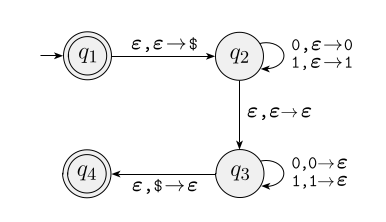
\includegraphics[width=0.5\textwidth]{images/ap3}
	\end{center}

\begin{enumerate}
\item $\epsilon$ \hspace*{0.5cm}{\color{red} {\bf Resposta: } Aceita, pois $q_1$ é estado final.}
\item $00$

\vspace*{0.3cm}

{\color{red} {\bf Resposta: } Aceita. A computação de um dos ramos do AP que aceita  00 é descrita a seguir:
	\begin{enumerate}
		\item Em $q_1$, o AP empilha o $\$$ e vai para $q_2$;
		\item Em $q_2$, o AP lê 0, empilha 0, e vai para $q_3$;
		\item Em $q_3$, o AP lê 0, desempilha 0, e continua em $q_3$;
		\item Em $q_3$, o AP desempilha o $\$$, e vai para $q_4$, aceitando a cadeia.		
	\end{enumerate}}

\item $11$

\vspace*{0.3cm}

{\color{red} {\bf Resposta: } Aceita. A computação de um dos ramos do AP que aceita  11 é descrita a seguir:
	\begin{enumerate}
		\item Em $q_1$, o AP empilha o $\$$ e vai para $q_2$;
		\item Em $q_2$, o AP lê 1, empilha 1, e vai para $q_3$;
		\item Em $q_3$, o AP lê 1, desempilha 1, e continua em $q_3$;
		\item Em $q_3$, o AP desempilha o $\$$, e vai para $q_4$, aceitando a cadeia.		
\end{enumerate}}

\item $010$ \hspace*{0.5cm} {\color{blue} {\bf Resposta: } Não aceita.}

\end{enumerate}

\end{enumerate}

\end{document}